\section{Risultati e discussione: effetti degli elementi legnosi}
È stato osservato che il legno che non viene mobilitato dalle piene è quello posto a quote relative maggiori, ad esempio su zone di deposito o sulle isole \squarecite{Gurnell:2001-island-formation}.
\\
Ogni elemento è stato individuato tramite un pallino sulla mappa; se l'elemento è esteso su più celle delle immagini, come succede nella stragrande maggioranza dei casi per i tronchi lunghi metri e gli accumuli di legno, il medesimo elemento può essere mappato in punti diversi su immagini successive.
Questo può far sembrare che il legno si sia spostato, anche se questo deriva dalla digitalizzazione manuale (ad esempio un albero depositato su una barra può essere mappato a metà del tronco o sull'apparato radicale; se viene parzialmente sepolto da un anno all'altro la mappatura può essere diversa).
Dall'altra parte, è possibile che un legno sia stato rimpiazzato da un altro: in questo caso considerare che l'elemento sia il medesimo non è corretto; tuttavia l'approccio consente di elaborare molti punti in poco tempo.
\\
È possibile per le digitalizzazioni degli elementi legnosi del~2010-08 e~2013-10-22 osservare se i tronchi e gli accumuli che si sono spostati sotto una certa soglia si trovano sulle quote relative più elevate.
La soglia può variare da \SIrange[range-phrase = { a }]{0.5}{2.5}{\m} ed è stata scelta valutando qualitativamente le digitalizzazione in anni successivi.
\\
I grafici in \cref{graph:elementi-dem-detrended-distanza} mostrano i \emph{boxplot} dei punti che hanno il legno più vicino nella digitalizzazione successiva a distanza inferiore ad una serie di soglie; l'ultimo grafico mostra invece la quota dei punti che hanno il legno più lontano della soglia nella digitalizzazione seguente.
%
\begin{figure}
	\centering
	\tikzsetnextfilename{elementi_dem_detrended_distanza}
\begin{tikzpicture}
	\begin{groupplot}[
		group style = {
			group size = 3 by 1,
			y descriptions at = edge left,
			x descriptions at = edge bottom,
			horizontal sep = 0.1cm,
		},
		width = 0.38\textwidth,
		height = 0.4\textwidth,
		xlabel = {Distanza soglia \si{[\m]}},
		%xticklabel style = {font=\tiny},
		ylabel = {Quota relativa \si{[\m]}},
		boxplot/draw direction = y,
		ymax = 0.65,
		ymin = -0.55,
		%enlarge y limits = 0.05,
		grid = major,
	]
	\nextgroupplot[ % 2010/2013 elementi fermi
		width = 0.3\textwidth,
		title = {2010-08/2013-10-22},
		xtick = {1, 2},
		xticklabels = {$2$, $2.5$},
		]
		\addplot [
		        boxplot prepared = {
		                lower whisker = -0.142529,
		                lower quartile = -0.049205,
		                median = 0.042889,
		                upper quartile = 0.189542,
		                upper whisker = 0.327826,
		                },
		        ]
		        coordinates {}
				node[below, red!75!black] at (boxplot box cs: \boxplotvalue{lower whisker},0.5){\pgfmathprintnumber{7}};
		\addplot [
		        boxplot prepared = {
		                lower whisker = -0.096515,
		                lower quartile = 0.020497,
		                median = 0.163037,
		                upper quartile = 0.245633,
		                upper whisker = 0.278409,
		                },
		        ]
		        coordinates {}
				node[below, red!75!black] at (boxplot box cs: \boxplotvalue{lower whisker},0.5){\pgfmathprintnumber{11}};	
	%------------------------------------------------------
	\nextgroupplot[ % 2013/2014 elementi fermi
		width = 0.55\textwidth,
		title = {2013-10-22/2014-10-31},
		xtick = {1, 2, 3, 4, 5},
		xticklabels = {$0.5$, $1$, $1.5$, $2$, $2.5$},
		]
		\addplot [
		        boxplot prepared = {
		                lower whisker = 0.281042,
		                lower quartile = 0.385799,
		                median = 0.437347,
		                upper quartile = 0.528038,
		                upper whisker = 0.562563,
		                },
		        ]
		        coordinates {}
				node[below, red!75!black] at (boxplot box cs: \boxplotvalue{lower whisker},0.5){\pgfmathprintnumber{8}};
		\addplot [
		        boxplot prepared = {
		                lower whisker = -0.004163,
		                lower quartile = 0.187134,
		                median = 0.364044,
		                upper quartile = 0.468307,
		                upper whisker = 0.528088,
		                },
		        ]
		        coordinates {}
				node[below, red!75!black] at (boxplot box cs: \boxplotvalue{lower whisker},0.5){\pgfmathprintnumber{33}};
		\addplot [
		        boxplot prepared = {
		                lower whisker = -0.076253,
		                lower quartile = 0.124092,
		                median = 0.349297,
		                upper quartile = 0.458878,
		                upper whisker = 0.568133,
		                },
		        ]
		        coordinates {}
				node[below, red!75!black] at (boxplot box cs: \boxplotvalue{lower whisker},0.5){\pgfmathprintnumber{60}};
		\addplot [
		        boxplot prepared = {
		                lower whisker = -0.118472,
		                lower quartile = 0.050575,
		                median = 0.342194,
		                upper quartile = 0.451180,
		                upper whisker = 0.565715,
		                },
		        ]
		        coordinates {}
				node[below, red!75!black] at (boxplot box cs: \boxplotvalue{lower whisker},0.5){\pgfmathprintnumber{90}};
		\addplot [
		        boxplot prepared = {
		                lower whisker = -0.273404,
		                lower quartile = -0.001945,
		                median = 0.312073,
		                upper quartile = 0.446487,
		                upper whisker = 0.565771,
		                },
		        ]
		        coordinates {}
				node[below, red!75!black] at (boxplot box cs: \boxplotvalue{lower whisker},0.5){\pgfmathprintnumber{119}};
	%------------------------------------------------------
	\nextgroupplot[ % elementi spostati
		width = 0.3\textwidth,
		title = {Legno mobilitato},
		xlabel = {Digitalizzazioni},
		xtick = {1, 2},
		xticklabels = {10/13, 13/14},
		] % punti più distanti
		\addplot [
		        boxplot prepared = {
		                lower whisker = -0.451044,
		                lower quartile = -0.118087,
		                median = 0.065396,
		                upper quartile = 0.254933,
		                upper whisker = 0.454207,
		                },
		        ]
		        coordinates {};
		\addplot [
		        boxplot prepared = {
		                lower whisker = -0.381036,
		                lower quartile = -0.136173,
		                median = 0.120033,
		                upper quartile = 0.352123,
		                upper whisker = 0.534039,
		                },
		        ]
		        coordinates {};
	\end{groupplot}
\end{tikzpicture}

	\caption[\emph{boxplot} delle quote relative dove si trova il legno mobilitato]{\emph{boxplot} delle quote relative dove si trova il legno mobilitato nelle digitalizzazioni 2010-08/2013-10-22 (per le quali non ci sono punti con distanza minore di \SI{2}{\m}) e 2013-10-22/2014-10-31; l'ultimo grafico mostra la quota relativa del legno non mobilitato, la quale è praticamente costante per ogni soglia di distanza.
	I numeri in rosso indicano il numero di punti che definisce ogni \emph{boxplot}; per l'ultimo grafico il numero di punti è superiore a~\num{600}.}
	\label{graph:elementi-dem-detrended-distanza}
\end{figure}
%

All'aumentare della soglia ci sono più punti con distanza minima tra una digitalizzazione e la successiva minore della soglia stessa.
Per le digitalizzazioni 2010-08/2013-10-22 al di sotto della soglia di~\SI{2}{\m} i punti per ogni \emph{boxplot} sono molto pochi, da~3 a nessuno, e sono quindi stati scartati; il basso numero di punti può essere dovuto alle numerose ed intense piene che sono avvenute tra le due date, le quali hanno di sicuro mobilitato gran parte del legname presente.
Per le digitalizzazioni 2013-10-22/2014-10-31 ci sono~8 punti per la soglia più piccola di~\SI{0.5}{\m}, sufficienti per avere un \emph{boxplot} significativo.
\\
I legni che vengono mobilitati, cioè i punti che presentano distanza minima maggiore della soglia, mostrano tutti la stessa distribuzione per ogni soglia all'interno di ciascuna coppia di digitalizzazioni confrontate: praticamente a qualunque quota relativa un elemento legnoso può essere spostato oppure seppellito da depositi di ghiaia, così da non essere più visibile nella digitalizzazione successiva.
\\
Per il 2010-08/2013-10-22, i \emph{boxplot} dei punti con distanza superiore alla soglia si sovrappongono completamente a quelli con distanza inferiore alla soglia: non è possibile quindi avanzare altre ipotesi se non che, al passaggio di un gran numero di piene e di eventi importanti, il legno si sposta e che gli elementi che sembrano non essersi mobilitati in realtà sono stati rimpiazzati da altri elementi.
\\
Nelle mappe 2013-10-22/2014-10-31 al crescere della soglia di distanza massima i \emph{boxplot} si estendono verso quote minori, ma la mediana varia molto poco rimanendo circa costante ad una quota di~\SIrange[range-phrase = {-}, range-units = single]{0.3}{0.4}{\m}.
Inoltre c'è una discreta separazione tra i \emph{boxplot} delle distanze inferiori di~\SIrange[range-phrase = { e }]{0.5}{1}{\m} e il \emph{boxplot} del legno mobilitato.
Questi fatti fanno pensare che gli elementi legnosi individuati da quelle soglie siano i medesimi tra il~2013 e il~2014: le piccole piene avvenute ad inizio del~2014 possono aver spostato il legno a quote relative minori mentre il legno posto più in alto non è stato toccato.
Quest'ultimo ha la possibilità concreta di riprodursi vegetativamente ed essere il nucleo di formazione di nuove isole.
\\
I \emph{boxplot} nel grafico in \cref{graph:legno-wj-dem-detrended-distanza} mostrano la distribuzione delle quote del DEM detrended del~2013-10-22 per diverse soglie di distanza; in più, sono suddivisi gli elementi legnosi in tronchi e accumuli; infine, dalla digitalizzazione del~2013-10-22 sono considerati i tronchi che al~2014-10-31 hanno come punto più vicino un tronco, un accumulo (che potrebbe essersi formato con le piene tra le digitalizzazioni) o un elemento non riconoscibile (che potrebbe essere il tronco in parte sepolto), e gli accumuli che hanno come punto più prossimo un accumulo o un elemento non riconoscibile.
Inoltre, viene riportata la distribuzione per gli i tronchi e gli accumuli con punti nella digitalizzazione seguente dello stesso tipo e con distanza superiore alla soglia; poiché queste distribuzioni sono di fatto identiche per ogni soglia, ne viene riportata solo una.
\\
Non è riportata la soglia di~\SI{0.5}{\m} per i tronchi poiché sono presenti solo~2 punti.
Non viene riportato un grafico per il~2010-08 poiché il numero di punti risultanti da questa suddivisione non è sufficiente per avere \emph{boxplot} significativi.
%
\begin{figure}
	\centering
	\tikzsetnextfilename{legno_wj_dem_detrended_distanza}
\begin{tikzpicture}
	\begin{groupplot}[
		group style = {
			group size = 3 by 1,
			y descriptions at = edge left,
			x descriptions at = edge bottom,
			horizontal sep = 0.1cm,
		},
		width = 0.38\textwidth,
		height = 0.4\textwidth,
		xlabel = {Distanza soglia \si{[\m]}},
		%xticklabel style = {font=\tiny},
		ylabel = {Quota relativa \si{[\m]}},
		boxplot/draw direction = y,
		ymax = 0.65,
		ymin = -0.55,
		%enlarge y limits = 0.05,
		grid = major,
	]
	\nextgroupplot[ % tronchi fermi
		width = 0.4\textwidth,
		title = {Tronchi fermi},
		xtick = {1, 2, 3, 4},
		xticklabels = {$1$, $1.5$, $2$, $2.5$},
		]
		\addplot [
		        boxplot prepared = {
		                lower whisker = -0.122345,
		                lower quartile = 0.167450,
		                median = 0.364044,
		                upper quartile = 0.437347,
		                upper whisker = 0.505463,
		                },
		        ]
		        coordinates {}
		node[below, red!75!black] at (boxplot box cs: \boxplotvalue{lower whisker},0.5){\pgfmathprintnumber{11}};
		\addplot [
		        boxplot prepared = {
		                lower whisker = 0.009230,
		                lower quartile = 0.206680,
		                median = 0.366295,
		                upper quartile = 0.459583,
		                upper whisker = 0.562486,
		                },
		        ]
		        coordinates {}
		node[below, red!75!black] at (boxplot box cs: \boxplotvalue{lower whisker},0.5){\pgfmathprintnumber{20}};
		\addplot [
		        boxplot prepared = {
		                lower whisker = 0.023849,
		                lower quartile = 0.180000,
		                median = 0.368546,
		                upper quartile = 0.477074,
		                upper whisker = 0.565659,
		                },
		        ]
		        coordinates {}
		node[below, red!75!black] at (boxplot box cs: \boxplotvalue{lower whisker},0.5){\pgfmathprintnumber{31}};
		\addplot [
		        boxplot prepared = {
		                lower whisker = -0.002211,
		                lower quartile = 0.127937,
		                median = 0.366295,
		                upper quartile = 0.489052,
		                upper whisker = 0.598705,
		                },
		        ]
		        coordinates {}
		node[below, red!75!black] at (boxplot box cs: \boxplotvalue{lower whisker},0.5){\pgfmathprintnumber{40}};
	%------------------------------------------------------
	\nextgroupplot[ % accumuli fermi
		width = 0.45\textwidth,
		title = {Accumuli fermi},
		xtick = {1, 2, 3, 4, 5},
		xticklabels = {$0.5$, $1$, $1.5$, $2$, $2.5$},
		]
		\addplot [
		        boxplot prepared = {
		                lower whisker = 0.223950,
		                lower quartile = 0.338135,
		                median = 0.401688,
		                upper quartile = 0.528015,
		                upper whisker = 0.596982,
		                },
		        ]
		        coordinates {}
		node[below, red!75!black] at (boxplot box cs: \boxplotvalue{lower whisker},0.5){\pgfmathprintnumber{5}};
		\addplot [
		        boxplot prepared = {
		                lower whisker = -0.002197,
		                lower quartile = 0.187134,
		                median = 0.338135,
		                upper quartile = 0.468307,
		                upper whisker = 0.585327,
		                },
		        ]
		        coordinates {}
		node[below, red!75!black] at (boxplot box cs: \boxplotvalue{lower whisker},0.5){\pgfmathprintnumber{21}};
		\addplot [
		        boxplot prepared = {
		                lower whisker = -0.090182,
		                lower quartile = 0.044922,
		                median = 0.321091,
		                upper quartile = 0.455734,
		                upper whisker = 0.595441,
		                },
		        ]
		        coordinates {}
		node[below, red!75!black] at (boxplot box cs: \boxplotvalue{lower whisker},0.5){\pgfmathprintnumber{37}};
		\addplot [
		        boxplot prepared = {
		                lower whisker = -0.273062,
		                lower quartile = -0.004040,
		                median = 0.317734,
		                upper quartile = 0.448982,
		                upper whisker = 0.557741,
		                },
		        ]
		        coordinates {}
		node[below, red!75!black] at (boxplot box cs: \boxplotvalue{lower whisker},0.5){\pgfmathprintnumber{54}};
		\addplot [
		        boxplot prepared = {
		                lower whisker = -0.325058,
		                lower quartile = -0.062695,
		                median = 0.265747,
		                upper quartile = 0.438202,
		                upper whisker = 0.554756,
		                },
		        ]
		        coordinates {}
		node[below, red!75!black] at (boxplot box cs: \boxplotvalue{lower whisker},0.5){\pgfmathprintnumber{72}};
	%------------------------------------------------------
	\nextgroupplot[ % elementi spostati
		width = 0.3\textwidth,
		title = {Legno mobilitato},
		xtick = {1, 2},
		xlabel = {},
		xticklabels = {Tr., Acc.},
		]
		\addplot [ % 500+ punti
		        boxplot prepared = {
		                lower whisker = -0.362068,
		                lower quartile = -0.118015,
		                median = 0.153465,
		                upper quartile = 0.357452,
		                upper whisker = 0.508168,
		                },
		        ]
		        coordinates {};
		\addplot [ % 300+ punti
		        boxplot prepared = {
		                lower whisker = -0.431021,
		                lower quartile = -0.199493,
		                median = 0.098511,
		                upper quartile = 0.353210,
		                upper whisker = 0.569949,
		                },
		        ]
		        coordinates {};
	\end{groupplot}
\end{tikzpicture}

	\caption[\emph{boxplot} delle quote relative distinte per tronchi e accumuli legnosi]{\emph{boxplot} delle quote relative dove si trovano tronchi (Tr.) e accumuli (Acc.) nelle digitalizzazioni 2013-10-22/2014-10-31; dopo aver calcolato la distanza dell'elemento della stessa tipologia più vicino da un'immagine all'altra, sono stati considerati gli elementi con distanza inferiore alla soglia; con la soglia~\SI{0.5}{\m} sono stati individuati solo~\num{2} tronchi, numero poco significativo e quindi scartato.
	L'ultimo grafico mostra la distribuzione dei tronchi e degli accumuli con distanza tra le digitalizzazioni superiori alle soglie; dato che queste distribuzioni sostanzialmente non variano cambiando soglia, se ne riporta solo una.
	I numeri in rosso indicano il numero di punti che definisce ogni \emph{boxplot}; per l'ultimo grafico il numero di punti è di diverse centinaia.}
	\label{graph:legno-wj-dem-detrended-distanza}
\end{figure}
%
\\
Confrontando i numeri di punti che concorrono a formare ogni \emph{boxplot}, si vede come sia maggiore il numero di accumuli che non si mobilita rispetto ai tronchi: questi ultimi differiscono dagli accumuli in quanto a conformazione, modo in cui possono essere parzialmente sepolti, resistenza offerta alla corrente (\cref{fig:tronco-vs-accumulo}).
%
\begin{figure}
	\centering
	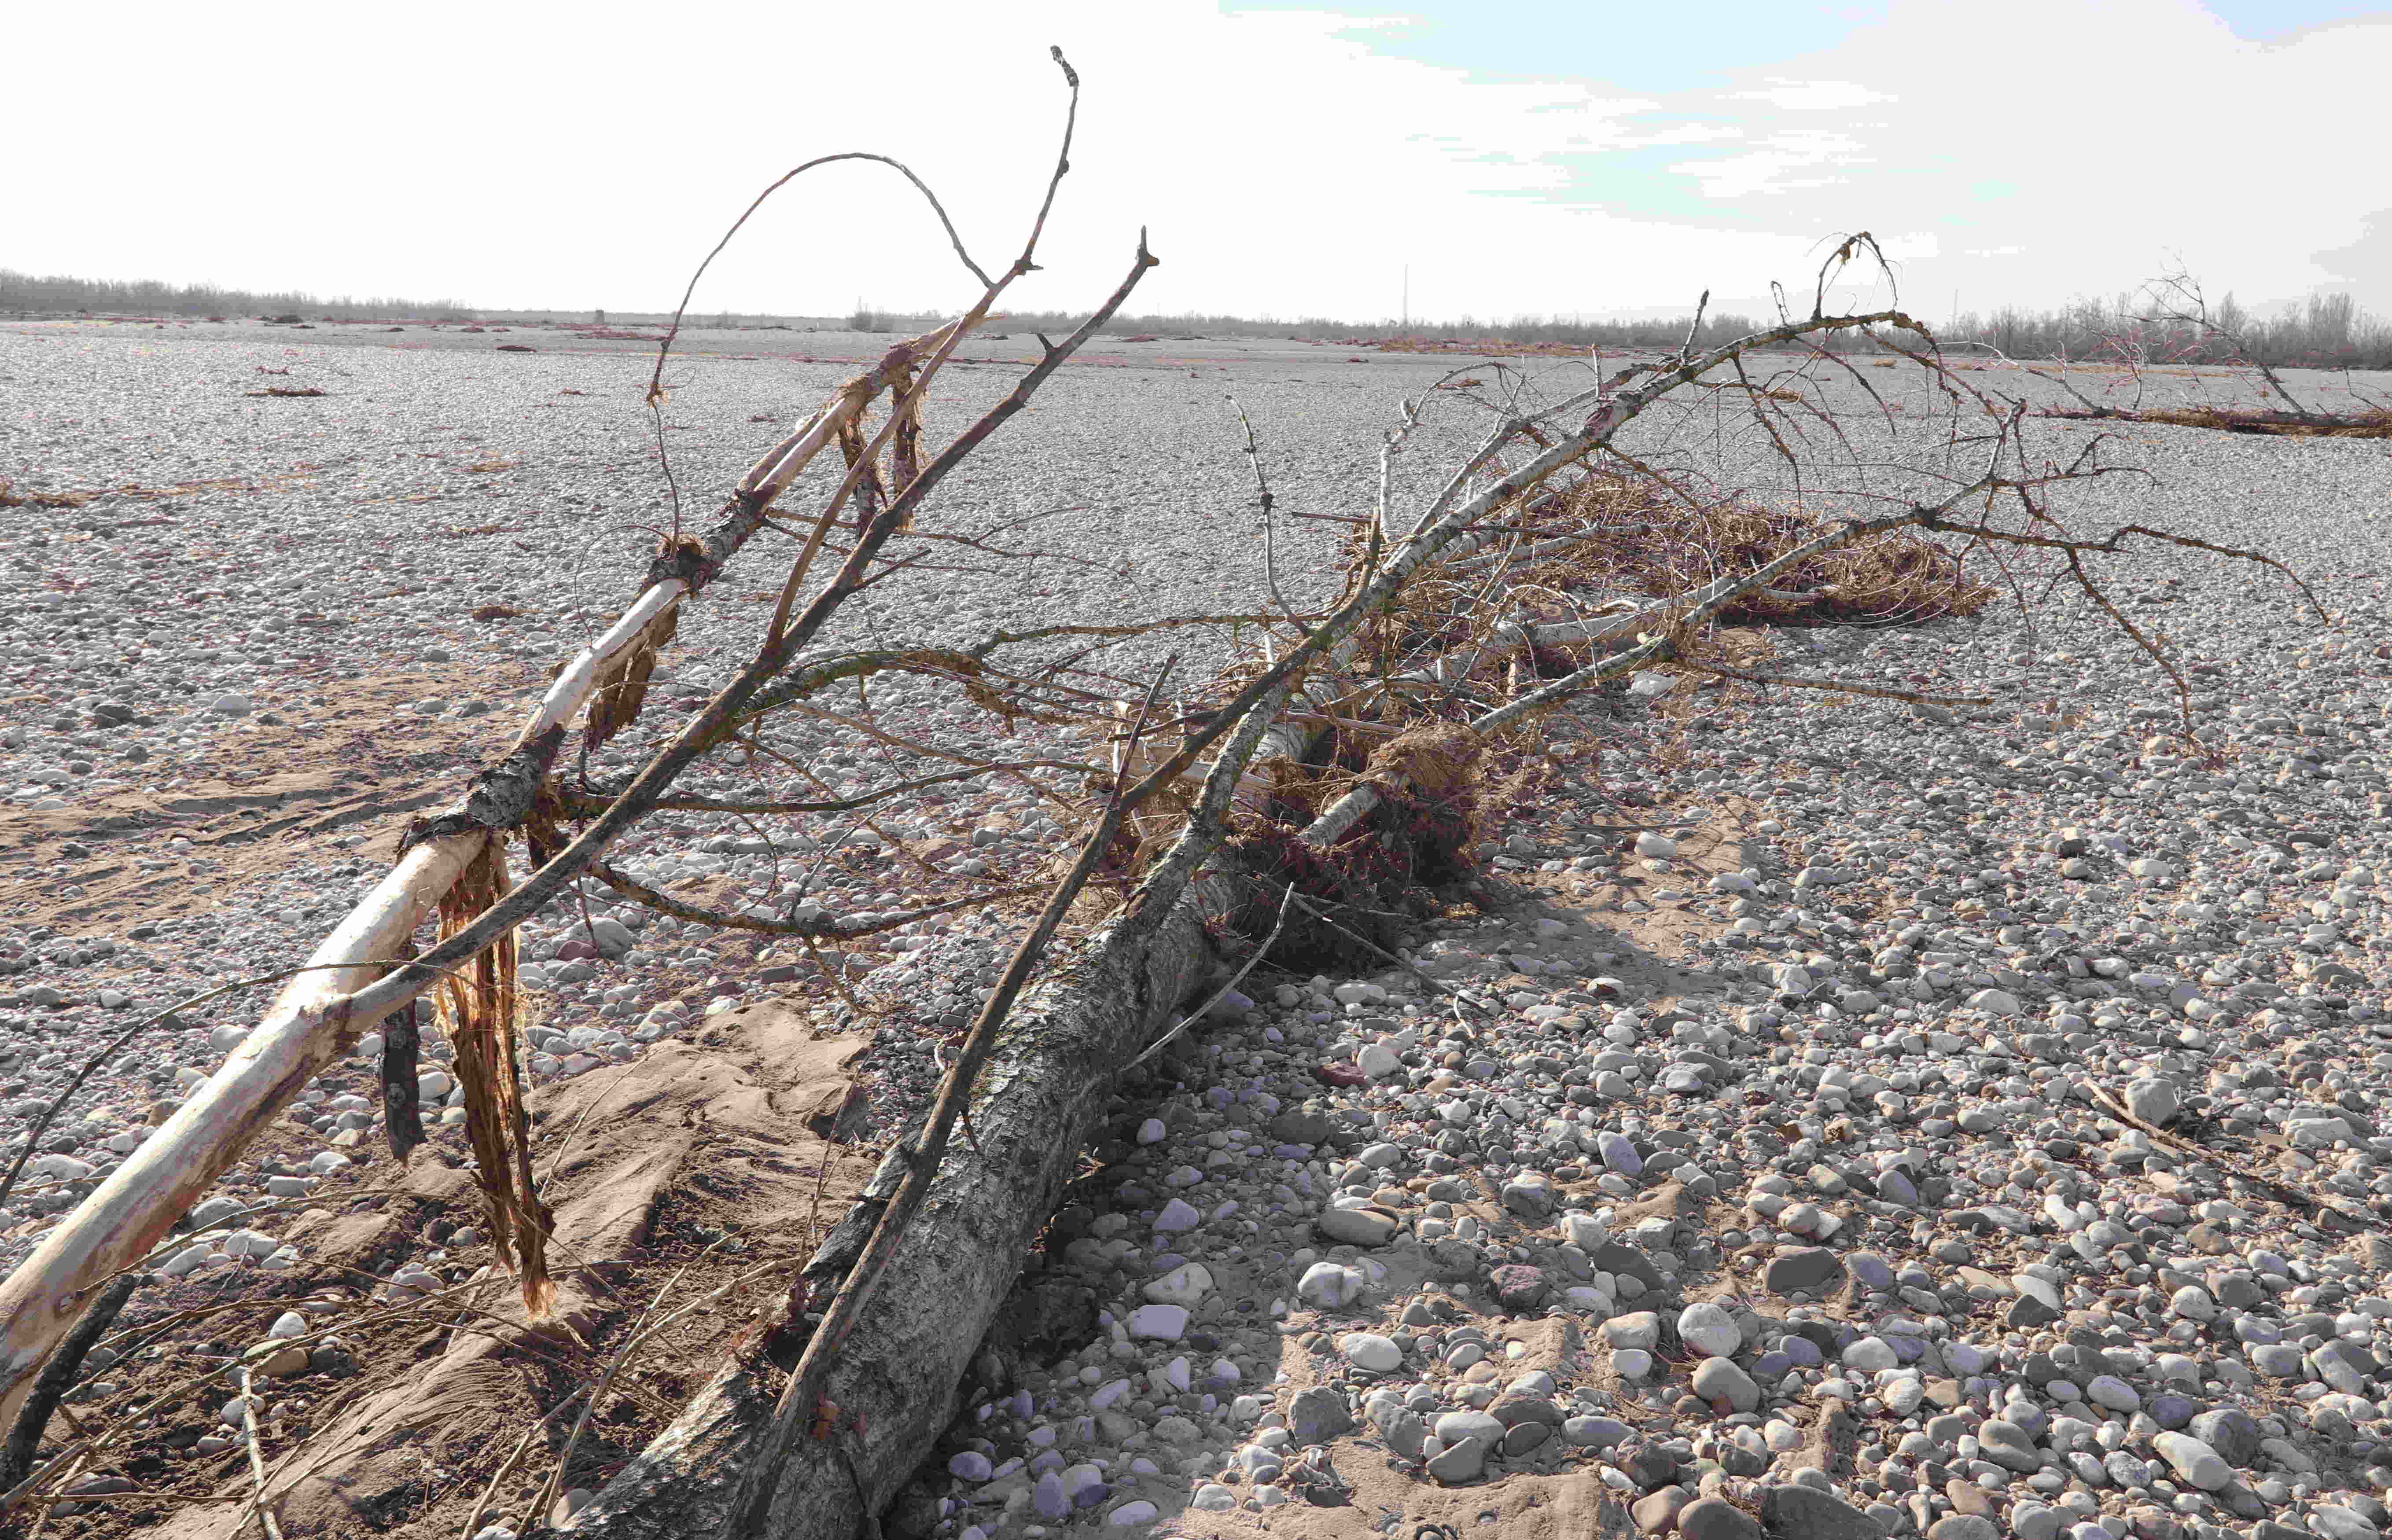
\includegraphics[height = 0.27\textwidth]{files/tronco.jpeg}
	\quad
	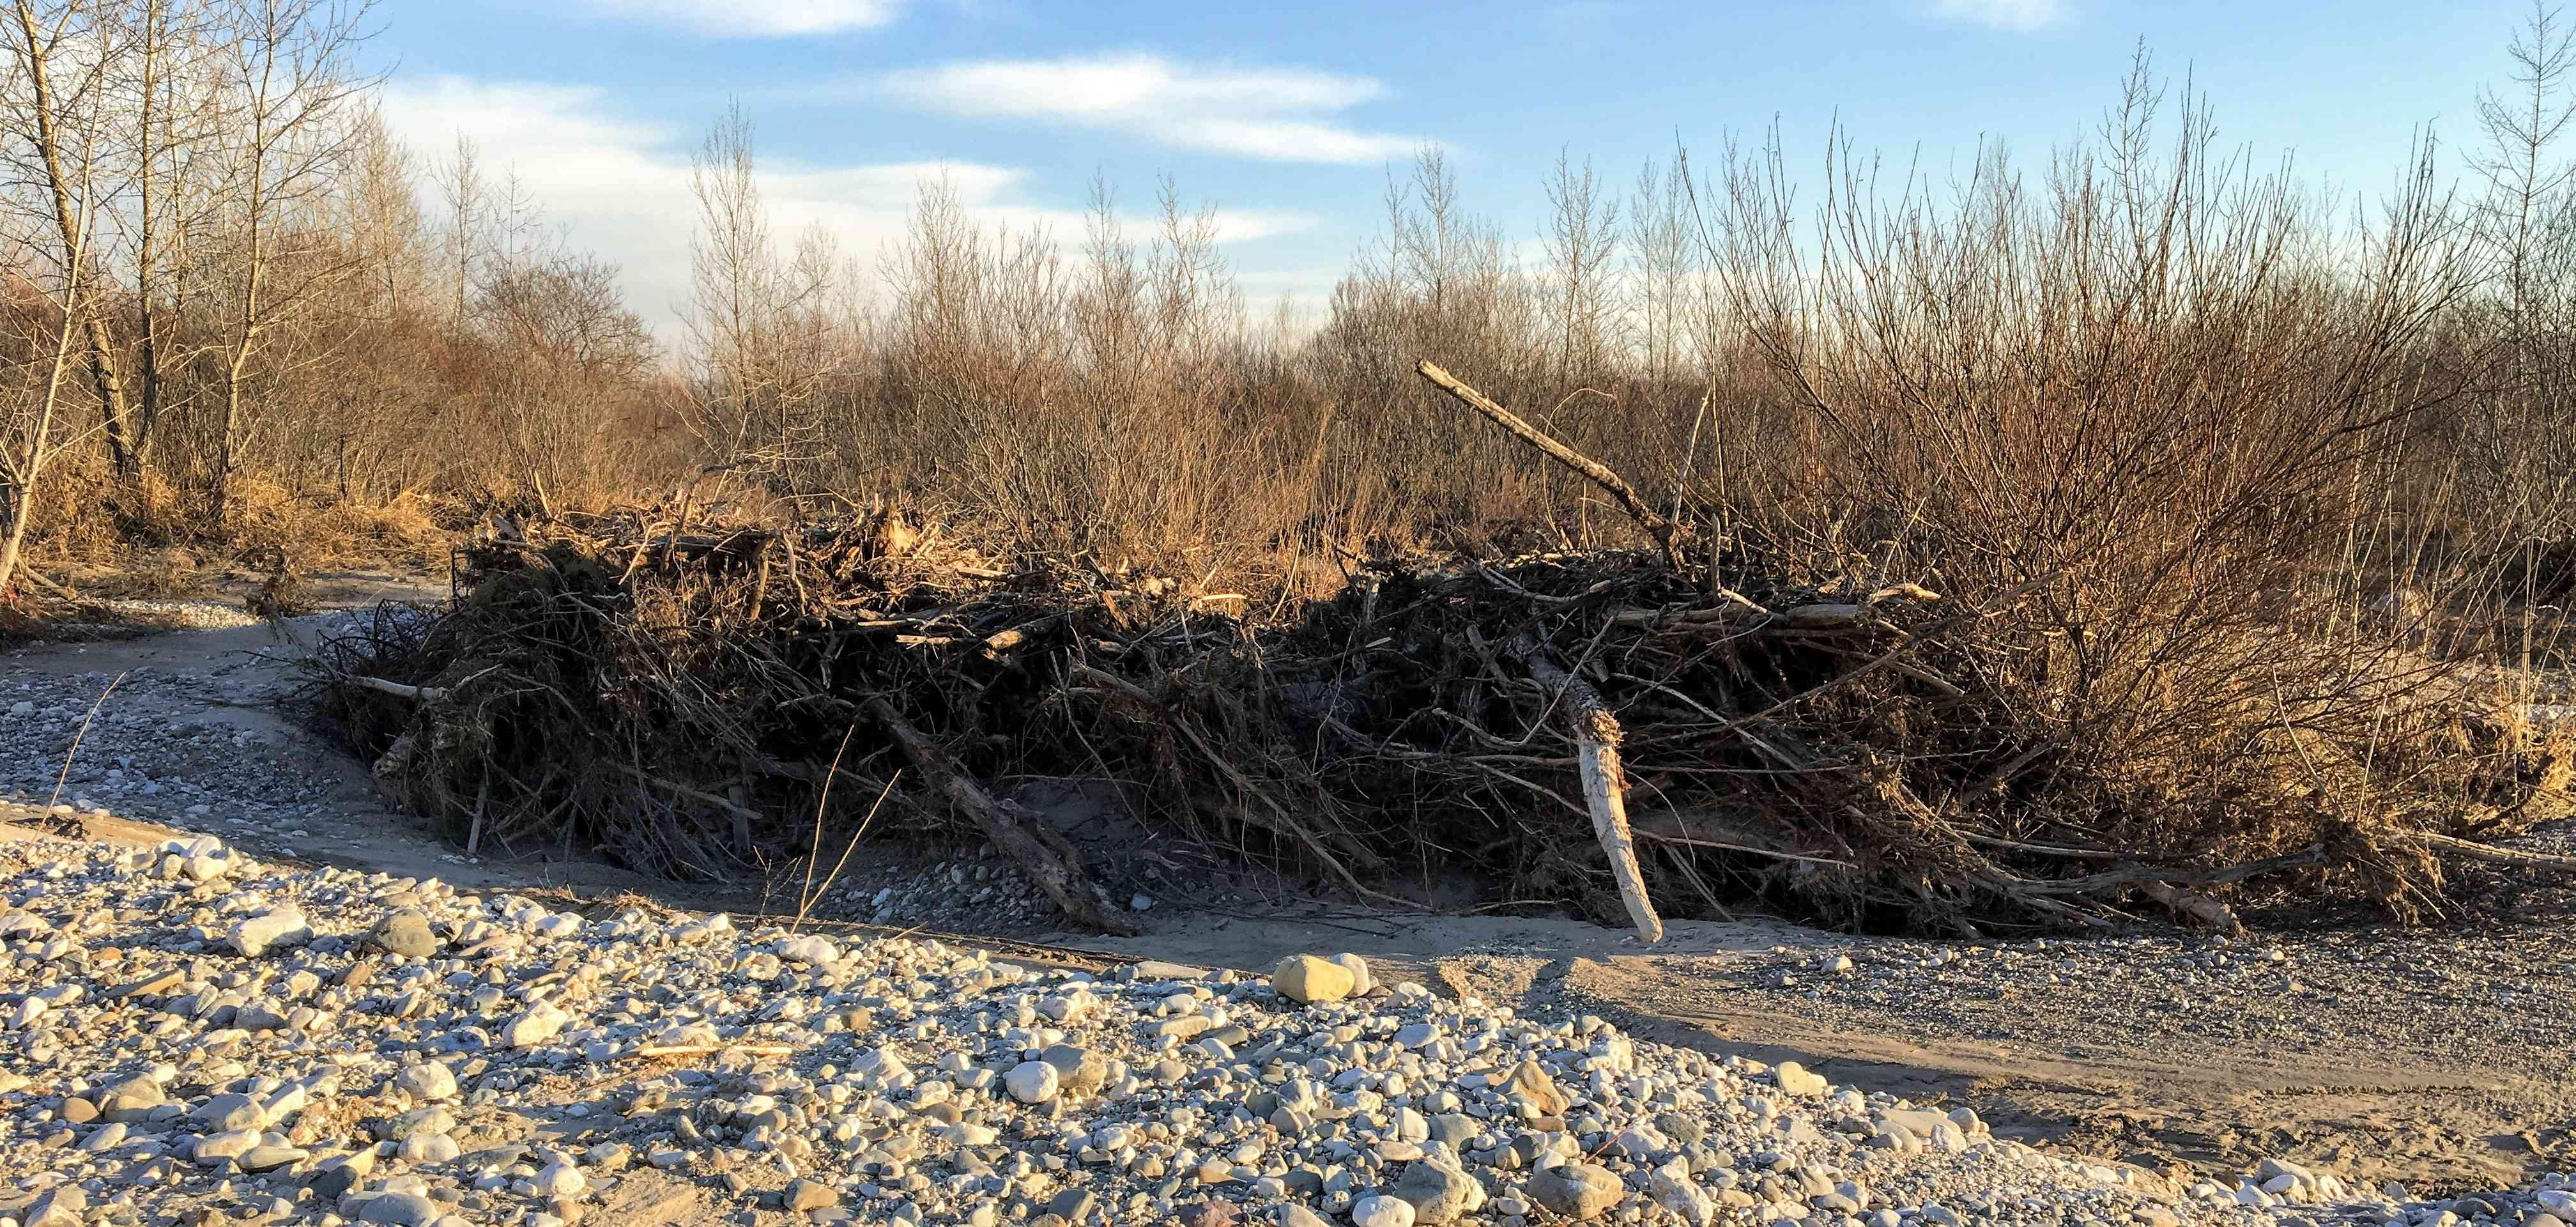
\includegraphics[height = 0.27\textwidth]{files/accumulo.jpeg}
	\caption[tronco depositato in alveo e accumulo vicino ad un'isola]{tronco depositato in alveo e accumulo vicino ad un'isola; foto scattate in data 2019-01-04 e 2019-01-05.}
	\label{fig:tronco-vs-accumulo}
\end{figure}
%
\\
La distribuzione degli accumuli, a differenza di quella dei tronchi, si allunga verso quote relative inferiori all'aumentare della distanza soglia; questo trend probabilmente è assente per i tronchi poiché questi possono resistere alle piene solo se sono stati depositati a quote elevate, mentre gli accumuli oppongono una resistenza minore.
È comprensibile quindi il motivo per cui i tronchi possono essere mobilitati più facilmente rispetto agli accumuli.
\\
Sia i tronchi che gli accumuli mantengono la mediana pressoché invariata a~\SIrange[range-phrase = {-}, range-units = single]{0.3}{0.4}{\m} per ogni soglia.
Il fatto che la mediana sia sempre superiore al terzo quartile dei \emph{boxplot} del legno mobilitato indica che gli elementi legnosi che non vengono spostati dalle piene sono quelli a quote relative più elevate, qualunque sia la tipologia di elemento.
\\
Questi risultati riflettono le numerosi osservazioni sul campo che sono state riportate da più articoli \squarecites{Gurnell:2001-island-formation}{Gurnell:2006-omega}{Bertoldi:2009-2m}{Gurnell:2014-plants-eng}.

La crescita è un fenomeno molto più lento dell'erosione ed è controllato da più fattori, come descritto nella sezione~\ref{sec:descr-area-studio}.
\\
Si è osservato tramite il confronto tra le digitalizzazioni 2014-10-31/2015-08-13 e 2015-08-13/2017 che molti degli elementi legnosi posti a quote relative elevate nel~2013-10-22 non si sono spostati fino agli anni più recenti; si è controllato se questi hanno gettato rami e foglie e se hanno formato delle isole pioniere.
Tuttavia, sembra che non ci sia stata alcuna crescita, forse a causa di una falda troppo profonda o di un substrato troppo grossolano; qualche pianta è cresciuta, ma pare che la successione biogeomorfica sia avanzata.
Dal controllo delle mappe che rilevano l'accrescimento delle isole utilizzate nelle sezioni precedenti non è stato notata alcuna nuova isola a partire da o attorno ai punti considerati.
\\
Da una parte molte piante sono cresciute a partire da semi in zone che già nell'ortofoto del~2005-05 si stavano vegetando. Il periodo 2005/2008 è stato molto favorevole per l'espansione delle isole, come già evidenziato nella sezione precedente.
Si può ipotizzare che queste isole abbiano occupato gran parte delle zone più aggradate; così non avrebbero consentito al nuovo legno di sfruttare le aree di ghiaia nuda adatte alla crescita (\cref{fig:crescita-2005-2010-2013}).
%
\begin{figure}
	\centering
	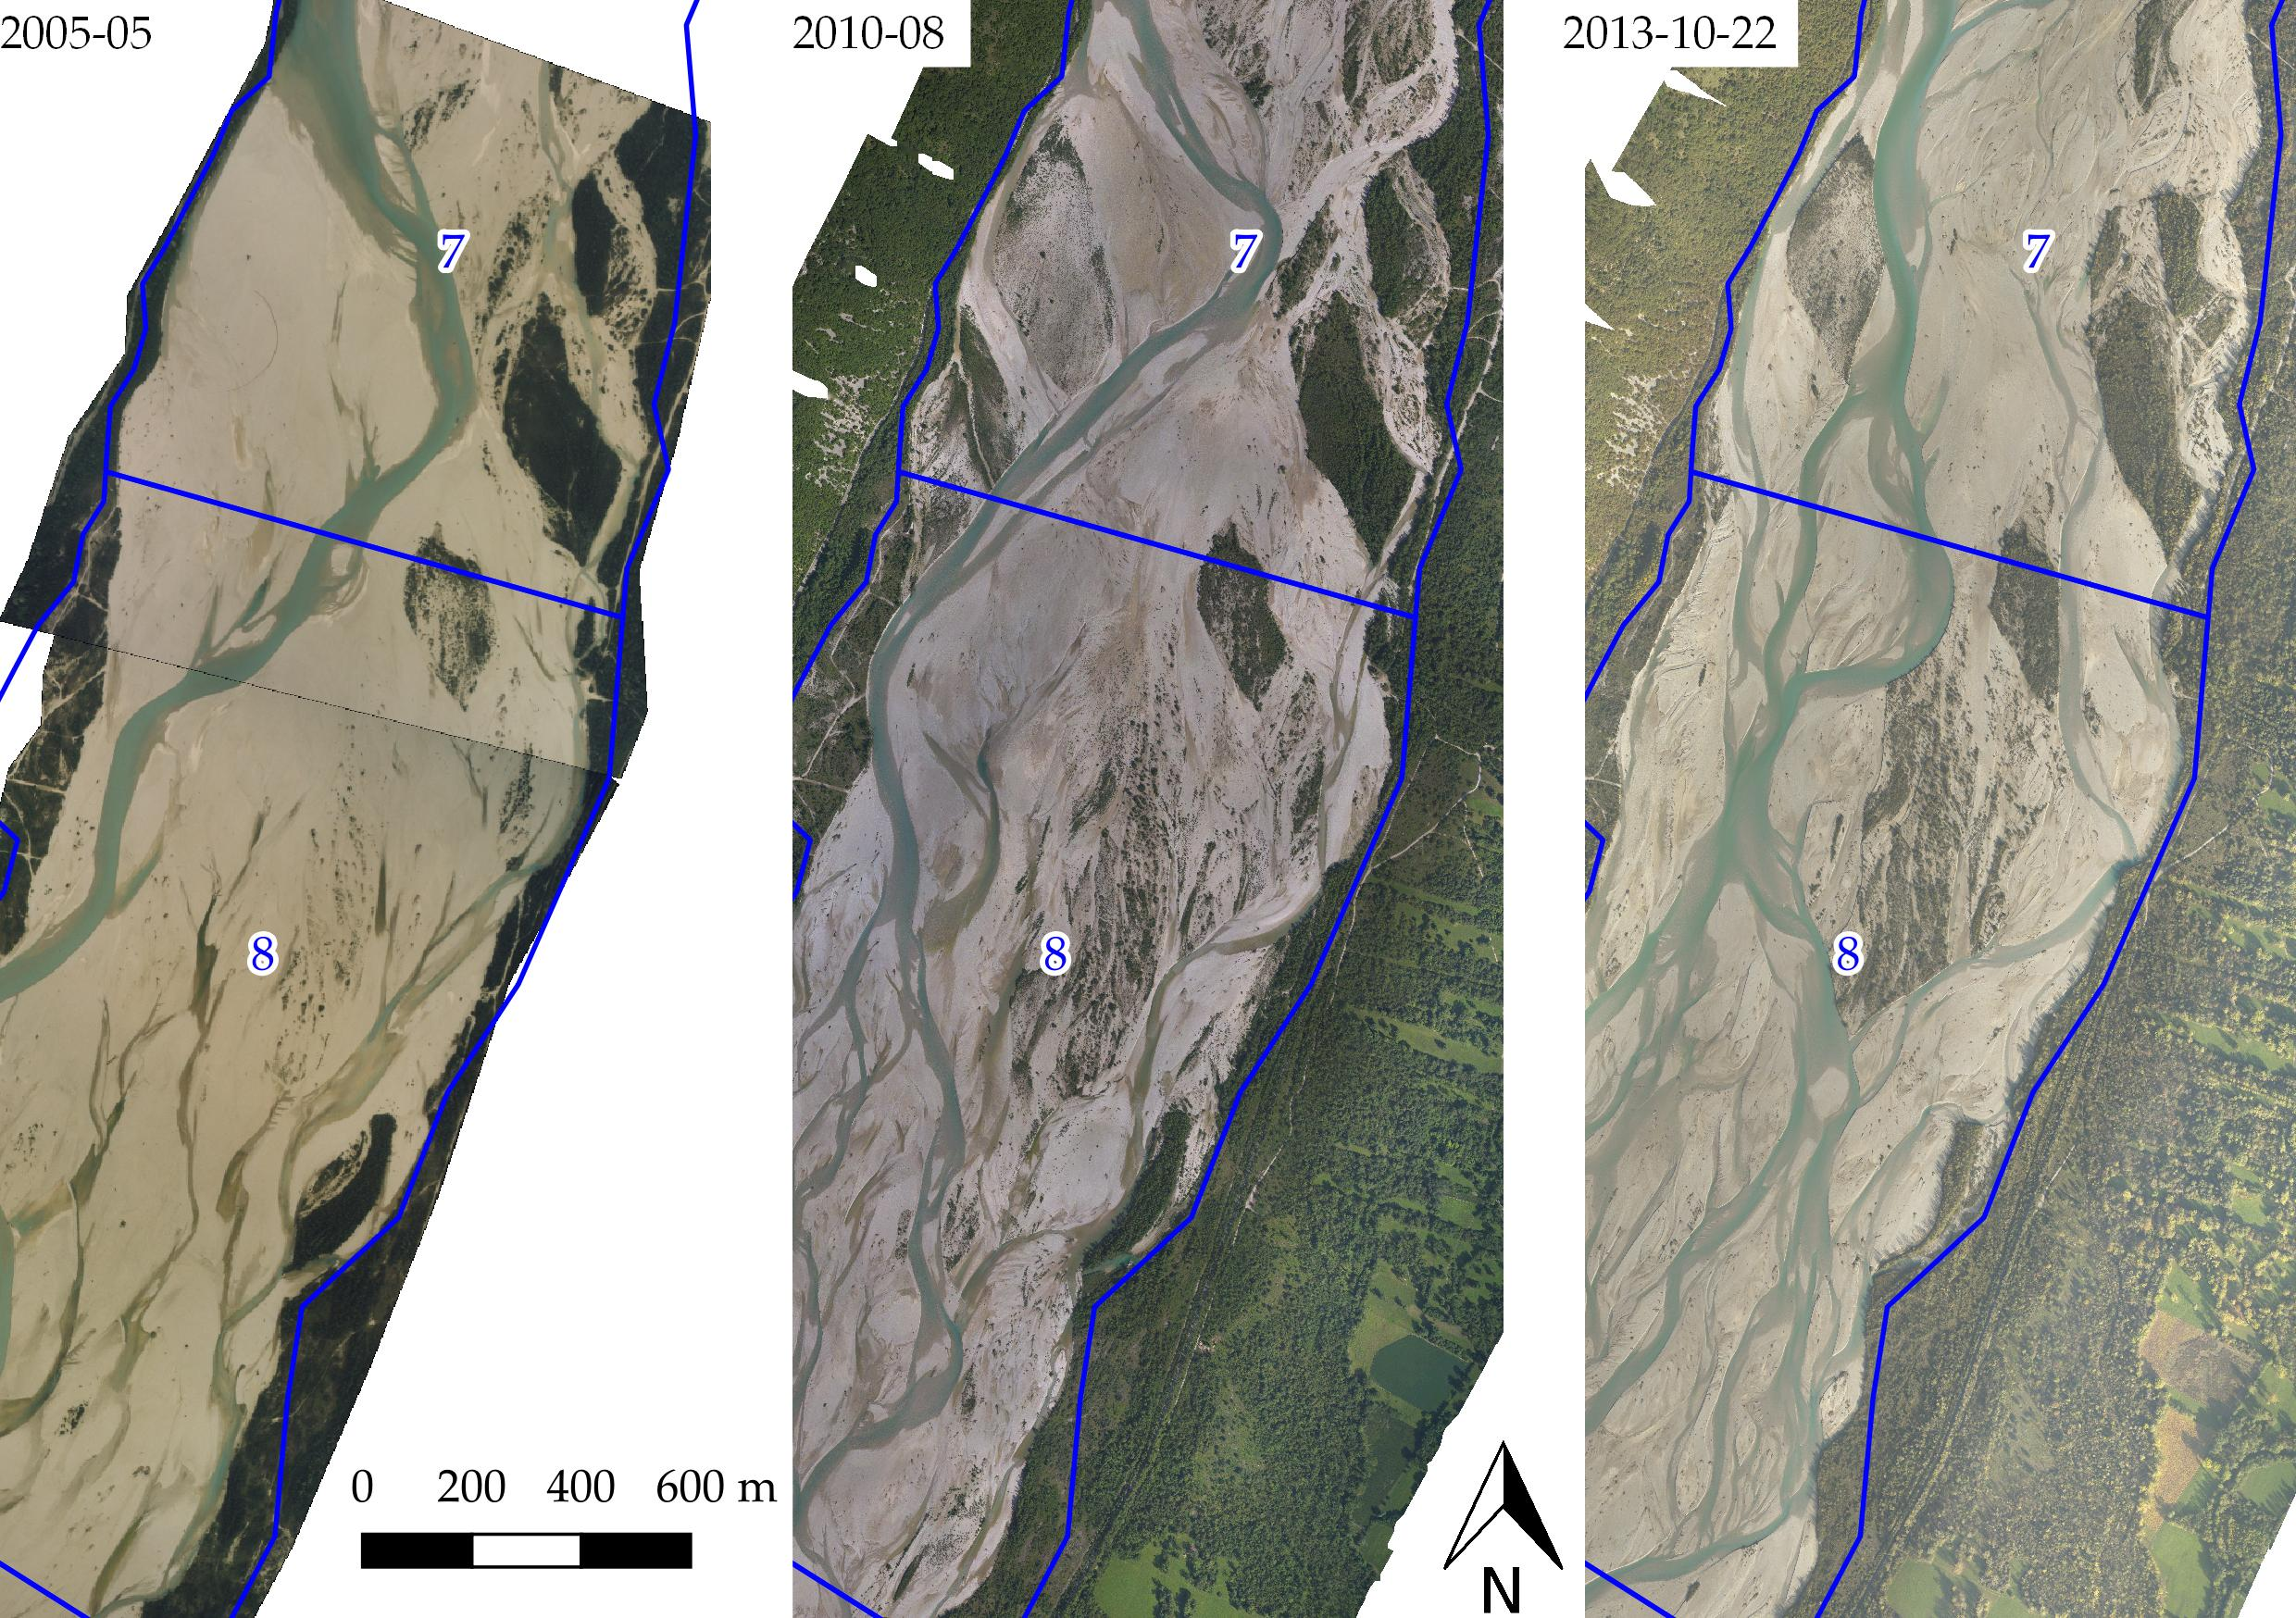
\includegraphics[width = \textwidth]{files/crescita_2005_2010_2013.jpeg}
	\caption[crescita delle isole nelle ortofoto 2005-05, 2010-08 e 2013-10-22]{crescita delle isole nelle ortofoto 2005-05, 2010-08 e 2013-10-22; si nota la forte colonizzazione di molte aree inizialmente di ghiaia nuda dal~2005-05 al~2010-08; in blu sono rappresentati i limiti della maschera computazionale divisa in tratti.}
	\label{fig:crescita-2005-2010-2013}
\end{figure}
%
